\documentclass[12pt, letterpaper, fleqn]{article}

% ----------------------------------------------------------
% PACKAGES
% ----------------------------------------------------------
\usepackage{graphicx}
\usepackage{xcolor}
\usepackage[most]{tcolorbox}
\usepackage{amsmath, amssymb}
\usepackage{fancyhdr}
\usepackage[utf8]{inputenc}
\usepackage[T1]{fontenc}
\usepackage{enumitem}
\usepackage{geometry}
\usepackage{tikz}
\usepackage{needspace}
\usepackage{booktabs}

\usetikzlibrary{arrows.meta, calc}

% ----------------------------------------------------------
% PAGE SETUP
% ----------------------------------------------------------
\usepackage{times}
\geometry{letterpaper, top=1.1in, bottom=1.1in, left=1in, right=1in, marginpar=0.5in}

% ----------------------------------------------------------
% HEADER / FOOTER
% ----------------------------------------------------------
\newcommand{\logowidth}{3cm}
\setlength{\headheight}{20pt}
\setlength{\footskip}{40pt}

\pagestyle{fancy}
\fancyhf{}
\fancyhead[C]{\small\bfseries 6th Grade Math Curriculum --- Comprehensive Placement Test}
\fancyfoot[L]{\raisebox{2pt}{
\includegraphics[width=\logowidth]{kss.png}}}
\fancyfoot[C]{\thepage}

\renewcommand{\footrulewidth}{0.2pt}

% ----------------------------------------------------------
% HELPER MACROS
% ----------------------------------------------------------
\newcommand{\blankshorter}{\underline{\hspace{2.0cm}}}
\newcommand{\blanklong}{\underline{\hspace{6.5cm}}}

% ----------------------------------------------------------
% DOCUMENT
% ----------------------------------------------------------
\begin{document}

\begin{center}
    {\LARGE \textbf{6th Grade Math Placement Test}}\\[4pt]
    {\large Diagnostic Assessment Across All 10 Curriculum Units}
\end{center}

\vspace{4mm}
\textbf{Name:} \underline{\hspace{6cm}}
\hfill
\textbf{Date:} \underline{\hspace{4cm}}\\
\vspace{2mm}

\begin{tcolorbox}[colback=black!5, colframe=black!40, arc=2mm, title=\textbf{Instructions for Students}]
This placement exam tests skills across all 5 major math domains of the 6th-grade curriculum. Read each problem carefully. Show your work for short-answer and multi-step questions to receive partial credit.
\end{tcolorbox}

\vspace{4mm}

% ==========================================================
% DOMAIN 1: RATIOS, RATES \& PROPORTIONS
% ==========================================================
\begin{tcolorbox}[colback=white, colframe=black, arc=2mm]
    \textbf{Domain 1: Ratios, Rates \& Proportions (Lessons 1--5)}
\end{tcolorbox}

\begin{enumerate}[leftmargin=0.6cm, itemsep=0.8cm]

\item \textbf{[Multiple Choice | Lesson 1]} A fruit basket contains $9$ apples and $12$ oranges. What is the ratio of apples to the \textbf{total} number of fruits in simplest form?
\begin{enumerate}[label=\Alph*)]
    \item $3:4$
    \item $4:3$
    \item $3:7$
    \item $4:7$
\end{enumerate}
\textbf{Answer Choice:} \blankshorter

\item \textbf{[Short Answer | Lesson 2]} A car travels $260$ miles in $4$ hours at a constant rate of speed. What is the car's unit rate of speed in miles per hour?
\\ \\
\textbf{Answer:} \blanklong

\item \textbf{[Short Answer | Lesson 3]} Complete the missing values in the equivalent ratio table below:
\begin{center}
\renewcommand{\arraystretch}{1.3}
\begin{tabular}{|l|c|c|c|}
\hline
\textbf{Blue Paint (cups)} & 3 & 6 & \blankshorter \\ \hline
\textbf{Yellow Paint (cups)} & 5 & \blankshorter & 20 \\ \hline
\end{tabular}
\end{center}

\item \textbf{[Short Answer | Lesson 4 \& 5]} A school track team has a goal to run $15$ miles this week. So far, they have completed $60\%$ of their goal.
\\ \\
\textbf{a)} How many miles have they run so far? \blankshorter \\ \\
\textbf{b)} Convert your answer from miles into yards. ($1\text{ mile} = 1,760\text{ yards}$).
\\ \\
\textbf{Answer:} \blanklong

\end{enumerate}
\vspace{0.5cm}

% ==========================================================
% DOMAIN 2: THE NUMBER SYSTEM \& FRACTIONS
% ==========================================================
\begin{tcolorbox}[colback=white, colframe=black, arc=2mm]
    \textbf{Domain 2: The Number System \& Fractions (Lessons 6--10)}
\end{tcolorbox}

\begin{enumerate}[leftmargin=0.6cm, itemsep=1.2cm, start=5]

\item \textbf{[Short Answer | Lesson 6]} Solve the fraction expression below. Write your final answer in its simplest fraction or mixed number form:
$$2\frac{1}{4} \div \frac{3}{8}$$
\vspace{1.5cm} \\
\textbf{Answer:} \blanklong

\item \textbf{[Short Answer | Lesson 7]} Solve each expression fluently:
\\ \\
\textbf{a)} $45.6 \times 1.25 =$ \blanklong \\ \\
\textbf{b)} Find the Greatest Common Factor (\textbf{GCF}) of $36$ and $54$: \blankshorter \\ \\
\textbf{c)} Find the Least Common Multiple (\textbf{LCM}) of $6$ and $8$: \blankshorter

\item \textbf{[Multiple Choice | Lesson 8 \& 10]} Consider the following statement about integers in real-world contexts: ``A bank account balance of $-\$45$ is deeper in debt than a balance of $-\$20$.'' Which absolute value inequality matches this reality?
\begin{enumerate}[label=\Alph*)]
    \item $|-45| > |-20|$
    \item $-45 > -20$
    \item $|-45| < |-20|$
    \item $-45 = -20$
\end{enumerate}
\textbf{Answer Choice:} \blankshorter

\item \textbf{[Short Answer | Lesson 9]} Write the ordered pair coordinates for the reflection of point $P(-3, 5)$ across the \textbf{y-axis}.
\\ \\
\textbf{Answer Point:} $(\ \blankshorter\ , \ \blankshorter\ )$

\end{enumerate}

\vspace{0.5cm}

% ==========================================================
% DOMAIN 3: EXPRESSIONS \& INTRO ALGEBRA
% ==========================================================
\begin{tcolorbox}[colback=white, colframe=black, arc=2mm]
    \textbf{Domain 3: Expressions \& Intro Algebra (Lessons 11--15)}
\end{tcolorbox}

\begin{enumerate}[leftmargin=0.6cm, itemsep=1.2cm, start=9]

\item \textbf{[Short Answer | Lesson 11]} Use the correct order of operations (PEMDAS) to evaluate the following numerical expression:
$$3^3 - (14 \div 2 + 5)$$
\vspace{1.5cm} \\
\textbf{Answer:} \blanklong

\item \textbf{[Short Answer | Lesson 12]} Evaluate the algebraic expression below when $x = 4$ and $y = 3.5$:
$$2x^2 + 4y - 3$$
\vspace{1.5cm} \\
\textbf{Answer:} \blanklong

\item \textbf{[Multiple Choice | Lesson 13]} Which of the following correctly demonstrates the distributive property to find an expression equivalent to $6(3x + 4)$?
\begin{enumerate}[label=\Alph*)]
    \item $18x + 4$
    \item $9x + 10$
    \item $18x + 24$
    \item $3x + 24$
\end{enumerate}
\textbf{Answer Choice:} \blankshorter

\item \textbf{[Long Answer | Lesson 14 \& 15]} An online bookstore charges a single baseline shipping flat fee of $\$4.50$ per delivery layout order, plus $\$3.00$ per book ($b$) purchased. 
\\ \\
\textbf{a)} Write an equation expressing the total cost ($C$) for an order of $b$ books.
\\ \\
\textbf{Equation:} \blanklong \\ \\
\textbf{b)} Identify which variable is the \textbf{independent variable} and which is the \textbf{dependent variable}:
\\ \\
\textbf{Independent:} \blanklong \quad \textbf{Dependent:} \blanklong \\ \\
\textbf{c)} Solve your equation to determine how many books were bought if a customer's total bill came out to exactly $\$22.50$. Show your balance steps.

\vspace{3cm}

\end{enumerate}

\vspace{0.5cm}

% ==========================================================
% DOMAIN 4: GEOMETRY \& MEASUREMENT
% ==========================================================
\begin{tcolorbox}[colback=white, colframe=black, arc=2mm]
    \textbf{Domain 4: Geometry \& Measurement (Lessons 16--20)}
\end{tcolorbox}

\begin{enumerate}[leftmargin=0.6cm, itemsep=1.2cm, start=13]

\item \textbf{[Short Answer | Lesson 16]} A triangle has a base length of $12\text{ cm}$ and a vertical height of $7.5\text{ cm}$. Find its area.
\\ \\
\textbf{Area:} \blanklong

\item \textbf{[Short Answer | Lesson 18]} A right rectangular prism storage container has a length of $6\text{ feet}$, a width of $2\frac{1}{2}\text{ feet}$, and a height of $4\text{ feet}$. Compute the total storage volume capacity inside the container in cubic feet.
\vspace{1.5cm} \\
\textbf{Volume:} \blanklong

\item \textbf{[Long Answer | Lesson 17 \& 20]} A small community playground landscape layout is plotted onto a coordinate map grid grid system where **each grid unit represents exactly $2\text{ yards}$**. The vertices of the rectangular plot are at:
$$A(-4, -2), \ B(5, -2), \ C(5, 4), \ \text{and } D(-4, 4)$$

\begin{center}
\begin{tikzpicture}[scale=0.5]
    \draw[lightgray, very thin] (-6,-4) grid (7,6);
    \draw[black, thick, -latex] (-6,0) -- (7,0) node[right, scale=0.8]{$x$};
    \draw[black, thick, -latex] (0,-4) -- (0,6) node[above, scale=0.8]{$y$};
    \foreach \x in {-4, 2, 4, 6} \draw (\x,0.1) -- (\x,-0.1) node[below, scale=0.6]{\x};
    \foreach \y in {-2, 2, 4} \draw (0.1,\y) -- (-0.1,\y) node[left, scale=0.6]{\y};
    
    \draw[thick, fill=purple!20] (-4,-2) rectangle (5,4);
    \node[below left, scale=0.7] at (-4,-2) {$A(-4,-2)$};
    \node[below right, scale=0.7] at (5,-2) {$B(5,-2)$};
    \node[above right, scale=0.7] at (5,4) {$C(5,4)$};
    \node[above left, scale=0.7] at (-4,4) {$D(-4,4)$};
\end{tikzpicture}
\end{center}

\textbf{a)} Determine the total length and width of the polygon boundary in **grid units**:
\\ \\
\textbf{Grid Length:} \blankshorter\ units \quad \textbf{Grid Width:} \blankshorter\ units \\ \\
\textbf{b)} Using the scale conversion factor ($1\text{ unit} = 2\text{ yards}$), determine the **actual** physical length and width dimensions in yards:
\\ \\
\textbf{Actual Length:} \blankshorter\ yards \quad \textbf{Actual Width:} \blankshorter\ yards \\ \\
\textbf{c)} Calculate the actual total field layout **area** of the playground in square yards.
\\ \\
\textbf{Area:} \blanklong

\end{enumerate}

\vspace{0.5cm}

% ==========================================================
% DOMAIN 5: STATISTICS, DATA \& MONEY
% ==========================================================
\begin{tcolorbox}[colback=teal!5, colframe=teal!60!black, arc=2mm]
    \textbf{Domain 5: Statistics, Data \& Money (Lessons 21--25)}
\end{tcolorbox}

\begin{enumerate}[leftmargin=0.6cm, itemsep=1.2cm, start=16]

\item \textbf{[Multiple Choice | Lesson 21]} Which of the following variations is a true \textbf{statistical question}?
\begin{enumerate}[label=\Alph*)]
    \item How tall is the school building in meters?
    \item How many inches did each student's science plant grow over the last three months?
    \item What is the maximum number of days in the month of October?
    \item Does $4 + 5$ equal $9$?
\end{enumerate}
\textbf{Answer Choice:} \blankshorter

\newpage

\item \textbf{[Short Answer | Lesson 22]} Find the mean and median values of this test score database setup: 
$$78, \ 85, \ 92, \ 65, \ 85$$
\vspace{1.5cm} \\
\textbf{Mean:} \blanklong \quad \textbf{Median:} \blanklong

\item \textbf{[Long Answer | Lesson 24 \& 25]} A student is creating a budget sheet for a school fundraiser event. They purchase a collection of layout decorations for an initial regular wholesale price of $\$120.00$. 
\\ \\
\textbf{a)} The party store offers a special single $15\%$ coupon discount off the decorations. Calculate the discount dollar savings and the resulting sale price.
\\ \\
\textbf{Discount Savings Amount:} \blanklong \\ \\
\textbf{Sale Price:} \blanklong \\ \\
\textbf{b)} The localized sales tax rate added onto the decoration check is $8\%$. Compute the final out-of-pocket cost of the decorations including the tax. Show your calculation steps.

\vspace{3cm}

\end{enumerate}

\end{document}
\end{document}